%======================================================================
\chapter{Implementation}
\label{ch:impl}

This chapter gives the algorithms behind each station, the loss functions used in training, the decision rules used at inference, the way the modules are integrated and deployed, and the tests that verify them. Long code listings are placed in Appendix~\ref{appendix:code}.

\section{Algorithm Implementation}
\label{sec:algorithm-implementation}

\subsection{Notation}
\label{sec:notation}
Table~\ref{tab:notation} collects the symbols used throughout this chapter.

\begin{table}[htbp]
\centering
\caption{Notation}
\label{tab:notation}
\begin{tabularx}{\textwidth}{|L{3.4cm}|X|}
\hline
\textbf{Symbol} & \textbf{Meaning} \\ \hline
$I_v \in \mathbb{R}^{H\times W\times 3}$ & Image from camera view $v\in\{1,2,3\}$ \\ \hline
$\mathcal{D}_v$ & Detections $\{(b_i,c_i,s_i,M_i)\}$ in view $v$: box $b_i=(x_1,y_1,x_2,y_2)$, class $c_i$, score $s_i$, mask $M_i$ \\ \hline
$\mathcal{C}$, $\mathcal{C}_d$ & Cap classes $\mathcal{C}=\{\text{good},\text{damaged},\text{misplaced},\text{no},\text{open},\text{wet}\}$; defect classes $\mathcal{C}_d=\mathcal{C}\setminus\{\text{good}\}$ \\ \hline
$F^T_\ell, F^S_\ell$ & Teacher and student feature maps at distillation site $\ell$ \\ \hline
$\phi_\ell$ & Learned $1{\times}1$ convolutional projector at site $\ell$ (training only) \\ \hline
$\alpha(t)$ & Distillation weight at epoch $t$ \\ \hline
$\tau_p,\tau_d,\tau_u$ & Cap gate thresholds: pass, defect, uncertain floor \\ \hline
$b$, $w$ & Bottle box $b=(x^b_1,y^b_1,x^b_2,y^b_2)$ and associated meniscus (water-surface) box $w$ \\ \hline
$h, h'$ & Bottle box height before and after trimming \\ \hline
$y_w$ & Meniscus height (box mid-line, clamped) \\ \hline
$\Rfill$ & Fill ratio, $0$ = empty, $1$ = full \\ \hline
$\theta_u,\theta_o,\beta,c_{\min}$ & Underfill and overfill limits, review half-band, minimum meniscus confidence \\ \hline
$T_k$, $\rho_k(x,y)$ & Template of label region $k$ and its normalised cross-correlation map \\ \hline
$A_k$, $\sigma_k$, $\tau_k$ & Anomaly map, anomaly score, and threshold of label region $k$ \\ \hline
\end{tabularx}
\end{table}

\subsection{Segmentation network}
\label{sec:seg-impl}
Both cap networks (teacher YOLO11x-seg and student YOLO11m-seg) share the YOLO11 segmentation design~\cite{jocher2024}. For an input image the backbone and neck produce feature maps at strides 8, 16, and 32. At every anchor point the head predicts (i) class logits $z\in\mathbb{R}^{|\mathcal{C}|}$, (ii) a discretised distribution over the four box-edge offsets, and (iii) a mask-coefficient vector $\mathbf{m}\in\mathbb{R}^{K}$. A separate prototype branch predicts $K=32$ full-image prototypes $P\in\mathbb{R}^{K\times H_p\times W_p}$. Following YOLACT~\cite{bolya2019}, the mask of instance $i$ is
\begin{equation}
    M_i = \sigma\!\left(\sum_{k=1}^{K} m_{i,k}\,P_k\right)\odot \mathbb{1}[b_i],
    \label{eq:mask}
\end{equation}
where $\sigma$ is the logistic function and $\mathbb{1}[b_i]$ crops the mask to the predicted box. Because the prototypes are shared, the per-instance cost of a mask is one $K$-dimensional linear combination.

\subsection{Supervised training loss}
The base loss is the Ultralytics segmentation loss, a weighted sum of four terms:
\begin{equation}
    \mathcal{L}_{\text{YOLO}} = \lambda_{\text{box}}\,\mathcal{L}_{\text{CIoU}} + \lambda_{\text{box}}\,\mathcal{L}_{\text{seg}} + \lambda_{\text{cls}}\,\mathcal{L}_{\text{BCE}} + \lambda_{\text{dfl}}\,\mathcal{L}_{\text{DFL}},
    \label{eq:yololoss}
\end{equation}
where $\mathcal{L}_{\text{CIoU}}$ is the complete-IoU box loss, $\mathcal{L}_{\text{seg}}$ is the per-pixel binary cross-entropy between predicted and ground-truth masks (normalised by box area and weighted by the box gain, as implemented in Ultralytics), $\mathcal{L}_{\text{BCE}}$ is the binary cross-entropy classification loss, and $\mathcal{L}_{\text{DFL}}$ is the distribution focal loss on the edge distributions. Positive anchors are chosen by a task-aligned assigner. We used $\lambda_{\text{box}}=7.5$, $\lambda_{\text{dfl}}=1.5$, and $\lambda_{\text{cls}}=4.0$.

The classification gain was raised from the default $0.5$ to compensate for class imbalance. With $n_c$ training instances of class $c$, the majority-to-class ratio averaged over classes is
\begin{equation}
    \bar{r} = \frac{1}{|\mathcal{C}|}\sum_{c\in\mathcal{C}}\frac{\max_{c'} n_{c'}}{n_c} = 6.29,
    \label{eq:imb}
\end{equation}
and the gain was set to $\min(\bar r, 4.0)=4.0$. This is a single scalar: it strengthens the classification signal relative to localisation but does not re-weight classes individually, unlike class-balanced or focal losses~\cite{cui2019,lin2017focal}.

\subsection{Teacher--student feature distillation}
\label{sec:kd-impl}

\noindent\textbf{General form.} A distillation objective for a detector can combine a response term, a box term, and a feature term:
\begin{equation}
    \mathcal{L}_{\text{distill}} = \alpha\,\mathcal{L}^{\text{KD}}_{\text{cls}} + \beta\,\mathcal{L}^{\text{KD}}_{\text{box}} + \gamma\,\mathcal{L}^{\text{KD}}_{\text{feat}}.
    \label{eq:distill-general}
\end{equation}
The response (logit) term matches temperature-softened class distributions~\cite{hinton2015},
\begin{equation}
    \mathcal{L}^{\text{KD}}_{\text{cls}} = \mathcal{T}^2\,\mathrm{KL}\!\left(\mathrm{softmax}(z^T/\mathcal{T})\,\Big\|\,\mathrm{softmax}(z^S/\mathcal{T})\right),
    \label{eq:logitkd}
\end{equation}
with temperature $\mathcal{T}>1$; the box term matches the teacher's edge distributions in the same way; and the feature term matches intermediate representations through learned projectors~\cite{romero2015}.

\noindent\textbf{Configuration used.} For bottle caps the decisive evidence (droplets, dents, a thread gap) covers a small part of the cap, and the teacher and student make near-identical final predictions on most images. Matching outputs alone would mainly transfer \emph{what} to predict. We therefore set $\alpha=\beta=0$ and distil features only, adding them to the supervised loss of Eq.~\eqref{eq:yololoss}:
\begin{equation}
    \mathcal{L} = \mathcal{L}_{\text{YOLO}} + \alpha(t)\sum_{\ell\in\mathcal{S}} \frac{1}{C_\ell H_\ell W_\ell}\left\| \widehat{F^T_\ell} - \widehat{\phi_\ell(F^S_\ell)} \right\|_2^2 ,
    \label{eq:kd}
\end{equation}
where $\mathcal{S}=\{\text{C3k2},\ \text{SPPF},\ \text{C2PSA}\}$ are the three distillation sites, $C_\ell\times H_\ell\times W_\ell$ is the teacher feature shape at site $\ell$, and $\widehat{\cdot}$ denotes channel-wise $L_2$ normalisation at every spatial position $(x,y)$:
\begin{equation}
    \widehat{F}(x,y) = \frac{F(x,y)}{\|F(x,y)\|_2+\epsilon}.
    \label{eq:l2norm}
\end{equation}

\noindent\textbf{Why normalise.} For unit vectors $\hat a$ and $\hat b$,
\begin{equation}
    \|\hat a-\hat b\|_2^2 = 2\left(1-\cos(a,b)\right),
    \label{eq:cosine}
\end{equation}
so the feature term of Eq.~\eqref{eq:kd} is a mean cosine distance between teacher and projected student features. It depends on the \emph{direction} of each feature vector and not on its magnitude, so the large, uniform background, where activations are strong but uninformative, cannot dominate the loss. This addresses the background-swamping problem noted for detector distillation~\cite{wang2019fgfi}.

\noindent\textbf{Distillation sites.} The three sites were chosen for what they carry. C3k2 at the backbone output holds edge and texture features, including thread and ridge geometry. SPPF at the backbone--neck transition holds multi-scale pooled context, which helps fine cues survive down-sampling. C2PSA holds the teacher's spatial attention, which transfers \emph{where} the fine defect evidence lies. The student and teacher feature maps have the same spatial size at each site because the two models share strides; only the channel widths differ. The projectors $\phi_\ell$ are $1{\times}1$ convolutions that lift student channels to teacher width ($256\rightarrow512$ and $512\rightarrow1024$).

\noindent\textbf{Schedule.} The distillation weight ramps linearly over the first 20 epochs:
\begin{equation}
    \alpha(t) = \alpha_0 + (\alpha_1-\alpha_0)\,\min\!\left(\frac{t}{t_r},1\right),\qquad \alpha_0=0.05,\ \alpha_1=0.5,\ t_r=20.
    \label{eq:ramp}
\end{equation}
Early epochs are dominated by the supervised loss, so the student first learns basic detection; the alignment pressure then reaches full strength. Teacher features are detached, so no gradient reaches the teacher. The projectors exist only in training and are discarded before export, so distillation adds no inference cost. Algorithm~\ref{alg:kd} summarises one training step.

\begin{algorithm}[htbp]
\caption{One training step of feature distillation}
\label{alg:kd}
\begin{algorithmic}[1]
\Require Batch $(X,Y)$, frozen teacher $f^T$, student $f^S$, projectors $\{\phi_\ell\}$, epoch $t$
\Ensure Updated student and projector parameters
\State Register forward hooks on sites $\ell\in\mathcal{S}$ in $f^T$ and $f^S$
\State $\{F^T_\ell\} \gets f^T(X)$ \textbf{without gradient} \Comment{teacher frozen}
\State $(\hat Y, \{F^S_\ell\}) \gets f^S(X)$
\State $\mathcal{L}_{\text{YOLO}} \gets$ Eq.~\eqref{eq:yololoss} on $(\hat Y, Y)$
\State $\mathcal{L}_{\text{feat}} \gets 0$
\For{each site $\ell\in\mathcal{S}$}
    \State $G \gets \phi_\ell(F^S_\ell)$ \Comment{$1{\times}1$ projection to teacher width}
    \State $\mathcal{L}_{\text{feat}} \gets \mathcal{L}_{\text{feat}} + \mathrm{MSE}\big(\mathrm{norm}(F^T_\ell),\ \mathrm{norm}(G)\big)$ \Comment{Eq.~\eqref{eq:l2norm}}
\EndFor
\State $\mathcal{L} \gets \mathcal{L}_{\text{YOLO}} + \alpha(t)\,\mathcal{L}_{\text{feat}}$ \Comment{Eq.~\eqref{eq:ramp}}
\State Back-propagate $\mathcal{L}$; update $f^S$ and $\{\phi_\ell\}$ with AdamW
\end{algorithmic}
\end{algorithm}

\noindent\textbf{Training configuration.} Table~\ref{tab:train-config} lists the settings. The teacher was trained first on the same data and settings at batch 16 for the full 150 epochs and then frozen. The student was initialised from COCO weights~\cite{lin2014coco}.

\begin{table}[htbp]
\centering
\caption{Training configuration of the cap teacher and student}
\label{tab:train-config}
\begin{tabularx}{\textwidth}{|L{3.6cm}|X|X|}
\hline
\textbf{Setting} & \textbf{Teacher (YOLO11x-seg)} & \textbf{Student (YOLO11m-seg)} \\ \hline
Parameters / GFLOPs @640 & 62.06\,M / 297.4 & 22.34\,M / 113.0 \\ \hline
Input size, batch & 640\,px, 16 & 640\,px, 32 \\ \hline
Optimiser & \multicolumn{2}{p{10.4cm}|}{AdamW, lr $10^{-3}\rightarrow10^{-5}$ cosine, 5 warm-up epochs, weight decay $5{\times}10^{-4}$} \\ \hline
Loss gains & \multicolumn{2}{p{10.4cm}|}{box 7.5, DFL 1.5, cls 4.0} \\ \hline
Augmentation & \multicolumn{2}{p{10.4cm}|}{mosaic (off for last 10 epochs), copy-paste 0.5, mixup 0.15, rotation $\pm15^\circ$, translate 0.1, scale 0.5, flips (v 0.3, h 0.5), HSV jitter, RandAugment, erasing 0.4} \\ \hline
Distillation & --- & Eq.~\eqref{eq:kd}, sites C3k2/SPPF/C2PSA \\ \hline
Epochs (best) & 150 (139) & 126, early stop, patience 30 (96) \\ \hline
Wall-clock time & 12.2\,h & 5.3\,h \\ \hline
Hardware & \multicolumn{2}{p{10.4cm}|}{NVIDIA RTX A5000 24\,GB; mixed precision; seed 42} \\ \hline
\end{tabularx}
\end{table}

\subsection{Asymmetric multi-view quality gate}
\label{sec:gate-impl}
The cap engine runs with a confidence floor of $0.35$. Let $\mathcal{D}_v$ be the detections of view $v$ above the floor, $(c^\star_v, s^\star_v)$ the class and score of the top detection, and
\begin{equation}
    s^{d}_v = \max\{s_i : (b_i,c_i,s_i,M_i)\in\mathcal{D}_v,\ c_i\in\mathcal{C}_d\}
\end{equation}
the strongest defect score ($-\infty$ if none). The per-view verdict is
\begin{equation}
    g(v)=\begin{cases}
    \texttt{FAILED} & \mathcal{D}_v=\emptyset\\
    \texttt{REJECT} & s^{d}_v \geq \tau_d\\
    \texttt{PASS} & c^\star_v=\text{good},\ s^\star_v\geq\tau_p\\
    \texttt{UNCERTAIN} & \text{otherwise}
    \end{cases}
    \label{eq:gate}
\end{equation}
with defaults $\tau_d=0.45$, $\tau_p=0.75$, and an uncertain floor $\tau_u=0.40$ that labels a good-cap score in $[\tau_u,\tau_p)$ as borderline in the audit record. The bottle verdict aggregates the views with a strict precedence:
\begin{equation}
    G = \begin{cases}
    \texttt{REJECT} & \exists v: g(v)=\texttt{REJECT}\\
    \texttt{INSPECTION\_FAILED} & \text{else } \exists v: g(v)=\texttt{FAILED}\\
    \texttt{UNCERTAIN} & \text{else } \exists v: g(v)=\texttt{UNCERTAIN}\\
    \texttt{PASS} & \text{otherwise.}
    \end{cases}
    \label{eq:agg}
\end{equation}
\texttt{REJECT} and \texttt{INSPECTION\_FAILED} fire the actuator; \texttt{UNCERTAIN} goes to the review queue without ejection. The thresholds are asymmetric by design ($\tau_d<\tau_p$): the bar for rejecting is lower than the bar for passing, so a doubtful cap is never passed automatically. All three thresholds can be changed at run time from the dashboard.

\subsection{Station 1 inspection cycle}
\label{sec:cap-cycle}
Algorithm~\ref{alg:capcycle} gives the complete Station 1 cycle for one bottle, from the three camera frames to the stored record and the dashboard update. It runs inside the cap service and calls the network of Section~\ref{sec:seg-impl} and the gate of Eqs.~\eqref{eq:gate}--\eqref{eq:agg}. The three views share one batched forward pass; if the loaded engine rejects a batch, the views are run one at a time so that the inspection still completes. Detections are taken from each view's own result, so NMS never mixes boxes from different cameras.

\begin{algorithm}[htbp]
\caption{Station 1 cap inspection cycle}
\label{alg:capcycle}
\begin{algorithmic}[1]
\Require Frames $\{I_v\}$ for $v\in\{\text{front},\text{rear},\text{side}\}$, cap engine $f$, thresholds $\tau_p,\tau_d,\tau_u$, confidence floor $0.35$
\Ensure Bottle verdict $G$, actuator flag, audit record
\State acquire the inference lock \Comment{one inspection per engine at a time}
\State $f \gets$ current engine reference, read once \Comment{a station switch may unload it}
\State $X \gets [I_{\text{front}}, I_{\text{rear}}, I_{\text{side}}]$, each resized to $640$\,px
\State $\{R_v\} \gets f(X)$ with confidence $\geq0.35$ \Comment{one batched pass}
\If{the engine rejects the batch}
    \State $R_v \gets f(I_v)$ for each view in turn \Comment{sequential fallback}
\EndIf
\For{each view $v$}
    \State $\mathcal{D}_v \gets$ boxes, classes, scores, and masks of $R_v$, rescaled to $I_v$ \Comment{per-view NMS}
    \State $g(v) \gets$ Eq.~\eqref{eq:gate} on $\mathcal{D}_v$
\EndFor
\State $G \gets$ Eq.~\eqref{eq:agg} on $\{g(v)\}$
\State actuator $\gets$ ($G=\texttt{REJECT}$ \textbf{or} $G=\texttt{INSPECTION\_FAILED}$)
\State write raw frames and YOLO labels to the bottle bundle; insert the \texttt{inspections} row and one \texttt{defect\_events} row per defect (SQLite, WAL)
\State render the per-view overlays and broadcast the result on the WebSocket stream
\State release the inference lock
\State \Return $G$, actuator, record
\end{algorithmic}
\end{algorithm}

\subsection{Fill-level estimation}
\label{sec:fill-impl}

\noindent\textbf{Stage 1: bottle localisation.} The bottle detector runs at confidence $\geq0.25$ and the highest-scoring \texttt{bottle} box $b$ is kept. If none is found the frame is treated as a conveyor gap.

\noindent\textbf{Stage 2: meniscus association and ratio.} The meniscus detector runs on the full frame at confidence $\geq0.15$. A candidate surface box $w=(x^w_1,y^w_1,x^w_2,y^w_2)$ is associated with the bottle when
\begin{equation}
    x^b_1 \leq \tfrac{1}{2}(x^w_1+x^w_2) \leq x^b_2
    \quad\wedge\quad
    \left(y^w_1\in[y^b_1,y^b_2] \ \vee\ y^w_2\in[y^b_1,y^b_2]\right),
    \label{eq:assoc}
\end{equation}
and among associated candidates the highest-scoring one is kept. With $h=y^b_2-y^b_1$, the bottle box is trimmed to remove detector padding at the cap and the base:
\begin{equation}
    y'_1 = y^b_1+\lfloor 0.03h\rfloor,\qquad y'_2 = y^b_2-\lfloor 0.02h\rfloor,\qquad h'=y'_2-y'_1 .
    \label{eq:trim}
\end{equation}
The meniscus height is the mid-line of the surface box, clamped to the trimmed bottle,
\begin{equation}
    y_w = \min\!\Big(y'_2,\ \max\!\big(y'_1,\ \lfloor (y^w_1+y^w_2)/2\rfloor\big)\Big),
\end{equation}
and the fill ratio is (image $y$ grows downwards)
\begin{equation}
    \Rfill = \frac{y'_2-y_w}{h'}\in[0,1].
    \label{eq:rfill}
\end{equation}
Figure~\ref{fig:fill-geom} illustrates the geometry.

\begin{figure}[htbp]
\centering
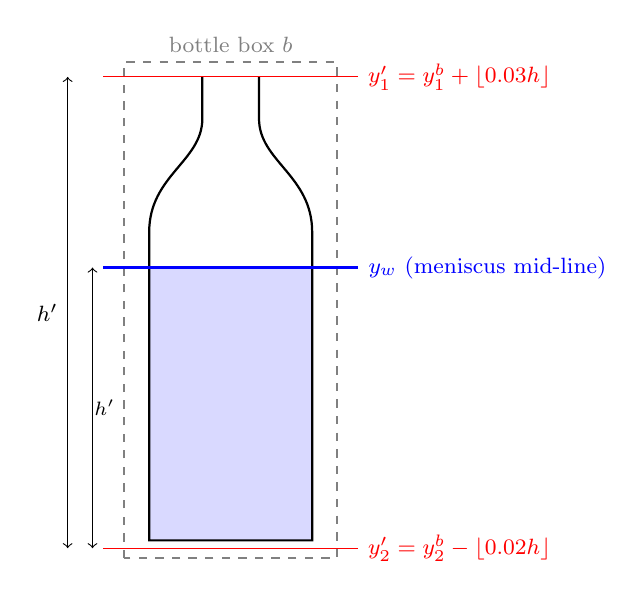
\begin{tikzpicture}[scale=0.9, every node/.style={font=\footnotesize}]
\draw[gray, dashed, thick] (0,0) rectangle (3,7);
\node[gray, above] at (1.5,7) {bottle box $b$};
\fill[blue!15] (0.35,0.25) rectangle (2.65,4.1);
\draw[thick] (1.1,6.8) -- (1.1,6.2) .. controls (1.1,5.6) and (0.35,5.4) .. (0.35,4.6) -- (0.35,0.25) -- (2.65,0.25) -- (2.65,4.6) .. controls (2.65,5.4) and (1.9,5.6) .. (1.9,6.2) -- (1.9,6.8);
\draw[red] (-0.3,6.79) -- (3.3,6.79) node[right]{$y'_1=y^b_1+\lfloor0.03h\rfloor$};
\draw[red] (-0.3,0.14) -- (3.3,0.14) node[right]{$y'_2=y^b_2-\lfloor0.02h\rfloor$};
\draw[blue, thick] (-0.3,4.1) -- (3.3,4.1) node[right]{$y_w$ (meniscus mid-line)};
\draw[<->] (-0.8,0.14) -- node[left]{$h'$} (-0.8,6.79);
\draw[<->] (-0.45,0.14) -- node[right, xshift=-1mm]{\scriptsize$\Rfill h'$} (-0.45,4.1);
\end{tikzpicture}
\caption{Fill-ratio geometry: trimmed bottle box (red) and meniscus mid-line (blue).}
\label{fig:fill-geom}
\end{figure}

\noindent\textbf{Stage 3: three-class fill state and gate.} The ratio is mapped to a fill state with the configurable limits $\theta_u=0.40$ and $\theta_o=0.85$:
\begin{equation}
    \text{state}(\Rfill) = \begin{cases}
    \text{underfill} & \Rfill<\theta_u\\
    \text{overfill} & \Rfill>\theta_o\\
    \text{acceptable} & \text{otherwise.}
    \end{cases}
    \label{eq:fillstate}
\end{equation}
These limits are engineering defaults, not regulatory values; they are read from a single configuration source so that a plant can set them per product, and the gate, the overlay ruler, and the health endpoint all read the same values. Algorithm~\ref{alg:fillgate} applies a review band of half-width $\beta=0.02$ around each limit when the meniscus confidence $c_w$ is below $c_{\min}=0.50$.

\begin{algorithm}[htbp]
\caption{Fill gate}
\label{alg:fillgate}
\begin{algorithmic}[1]
\Require Bottle box $b$ (or none), meniscus box $w$ with confidence $c_w$ (or none), $\Rfill$
\Ensure Verdict $V$ and actuator flag
\If{no bottle}
    \State \Return \texttt{INSPECTION\_FAILED}, no actuation \Comment{conveyor gap}
\ElsIf{no associated meniscus}
    \State \Return \texttt{REJECT} \Comment{empty or opaque}
\ElsIf{$\min_{\theta\in\{\theta_u,\theta_o\}}|\Rfill-\theta|\leq\beta$ \textbf{and} $c_w<c_{\min}$}
    \State \Return \texttt{UNCERTAIN} \Comment{borderline and weakly detected}
\ElsIf{state$(\Rfill)\neq$ acceptable}
    \State \Return \texttt{REJECT} (underfill or overfill)
\Else
    \State \Return \texttt{PASS}
\EndIf
\end{algorithmic}
\end{algorithm}

\noindent\textbf{Sensitivity.} Differentiating Eq.~\eqref{eq:rfill} gives
\begin{equation}
    \frac{\partial \Rfill}{\partial y_w} = -\frac{1}{h'},\qquad
    \frac{\partial \Rfill}{\partial y'_1} = \frac{\Rfill}{h'},\qquad
    \frac{\partial \Rfill}{\partial y'_2} = \frac{1-\Rfill}{h'}.
    \label{eq:sens}
\end{equation}
An error of $\delta$ pixels in the meniscus shifts the ratio by $\delta/h'$. For the median test bottle ($h=620$\,px, $h'\approx589$\,px) one pixel is $0.0017$, so the $\pm0.02$ review band corresponds to about 12 pixels. If the three edge errors are independent with standard deviations $\sigma_w$, $\sigma_1$, and $\sigma_2$, first-order propagation gives
\begin{equation}
    \sigma_R \approx \frac{1}{h'}\sqrt{\sigma_w^2 + \Rfill^2\sigma_1^2 + (1-\Rfill)^2\sigma_2^2}.
    \label{eq:prop}
\end{equation}
Using the mid-line of the surface box rather than one of its edges halves the effect of a symmetric error in the box height, because both edges move by equal and opposite amounts.

\noindent\textbf{Why a rule rather than a classifier.} A MobileNetV3 fill-level classifier was also trained during the project and reached 93.10\% test accuracy (135 of 145 images). It is not used in the deployed path: a classifier returns a label but no measurement, so its limits cannot be moved per product without retraining, and its errors cannot be traced to a pixel position. The geometric rule exposes $\Rfill$, its limits, and its sensitivity.

\subsection{Label-defect prototype}
\label{sec:label-impl}

\noindent\textbf{Preprocessing and localisation.} The scan $I$ is converted to grayscale. For each region $k$ a full-resolution template $T_k$ was cut from one clean reference scan. The match score at offset $(x,y)$ is the zero-mean normalised cross-correlation~\cite{lewis1995}
\begin{equation}
    \rho_k(x,y) = \frac{\sum_{u,v}\tilde T_k(u,v)\,\tilde I(x+u,y+v)}
    {\sqrt{\sum_{u,v}\tilde T_k(u,v)^2\ \sum_{u,v}\tilde I(x+u,y+v)^2}}\in[-1,1],
    \label{eq:ncc}
\end{equation}
where $\tilde{\cdot}$ subtracts the mean over the template window. Search is coarse-to-fine: Eq.~\eqref{eq:ncc} is evaluated on the image and template down-sampled by 4, and the peak is refined at full resolution within $\pm12$ pixels. Because the label wraps around the tube, each region occurs twice; candidates whose region would extend past the scan are discarded so that the complete occurrence is kept. A region is \emph{missing} when its best score is below $0.45$. If two located regions overlap by more than 10\% of the smaller one, the lower-scoring region is searched again with the other's area excluded, so that a damaged region is reported missing instead of silently landing on a neighbour.

\noindent\textbf{ROI cropping.} Each located region is cropped and rotated $90^\circ$ clockwise into the upright orientation in which the anomaly models were trained, then resized to $256{\times}256$. For the grayscale models the single channel is replicated to three channels.

\noindent\textbf{Model routing and anomaly scoring.} Each crop is routed to the EfficientAD-Medium model of its region~\cite{batzner2024}. EfficientAD has a frozen pretrained teacher network $\mathcal{T}$, a student $\mathcal{S}$ with two output groups, and an autoencoder $\mathcal{A}$, all trained only on good crops. For a crop $x$ the two anomaly maps are
\begin{equation}
    A^{\text{ST}}(x) = \frac{1}{C}\sum_{c}\big(\mathcal{T}_c(x)-\mathcal{S}^{\text{st}}_c(x)\big)^2,\qquad
    A^{\text{AE}}(x) = \frac{1}{C}\sum_{c}\big(\mathcal{A}_c(x)-\mathcal{S}^{\text{ae}}_c(x)\big)^2,
\end{equation}
the first sensitive to local texture anomalies and the second to logical or layout anomalies. Each map is normalised with statistics from good validation crops and the two are averaged into $A_k(x)$. The region score is the mean of the map,
\begin{equation}
    \sigma_k = \frac{1}{|\Omega|}\sum_{p\in\Omega} A_k(x)_p ,
    \label{eq:roiscore}
\end{equation}
and the label verdict is
\begin{equation}
    \text{label} = \begin{cases}
    \texttt{FAIL} & \exists k:\ \sigma_k>\tau_k \ \text{or region } k \text{ missing}\\
    \texttt{PASS} & \text{otherwise.}
    \end{cases}
    \label{eq:labelrule}
\end{equation}

\noindent\textbf{Threshold calibration.} Defective crops are used only to set thresholds. Two strategies were used: a recall-targeted threshold at the 5th percentile of defective-crop scores, which guarantees that at least 95\% of the calibration defects exceed it, and an F1-optimal sweep. For the final ROI\_4 model the crops were split 80/20 with a fixed seed; the threshold was set on the calibration part for a 95\% recall target and evaluated once on the remaining part.

\noindent\textbf{Explainability.} The upload-and-inspect application overlays the pixels of $A_k$ that exceed $\tau_k$, finds up to three connected hot regions, and reports for each how much it adds to $\sigma_k$ and what the region would score if that area were replaced by the crop median. If the counterfactual score falls below the threshold, that area alone causes the rejection. Algorithm~\ref{alg:label} summarises the prototype.

\begin{algorithm}[htbp]
\caption{Label-defect inspection}
\label{alg:label}
\begin{algorithmic}[1]
\Require Scan $I$, templates $\{T_k\}$, models $\{\mathcal{M}_k\}$, thresholds $\{\tau_k\}$
\Ensure Label verdict, per-region scores and heatmaps
\State $G \gets \mathrm{gray}(I)$; $G_4 \gets \mathrm{downsample}(G,4)$
\For{$k=1$ \textbf{to} $4$}
    \State $(x_k,y_k) \gets \arg\max \rho_k$ on $G_4$, complete occurrences only; refine on $G$ within $\pm12$\,px
    \State mark region $k$ missing if $\rho_k<0.45$
\EndFor
\State resolve overlaps $>10\%$ by re-searching the lower-scoring region
\For{each found region $k$}
    \State $x \gets \mathrm{resize}(\mathrm{rot90}(\mathrm{crop}(I,k)),256)$
    \State $A_k \gets \mathcal{M}_k(x)$;\ $\sigma_k \gets \mathrm{mean}(A_k)$
\EndFor
\State \Return Eq.~\eqref{eq:labelrule}, $\{\sigma_k\}$, $\{A_k\}$
\end{algorithmic}
\end{algorithm}

\section{System Integration}
\label{sec:system-integration}

\subsection{Pipeline per inspection}
Each Station 1 inspection runs ingestion, inference, quality gate, audit logging, and overlay rendering in that order (Figure~\ref{fig:integration-flow}). Overlays are rendered on demand from stored detections, so the stored images stay clean and can be re-used for training.

\begin{figure}[htbp]
\centering
\begin{adjustbox}{max width=\textwidth}
\begin{tikzpicture}[node distance=6mm, every node/.style={font=\footnotesize}]
\node[data, text width=2.2cm] (ing) {Ingestion\\(camera bundle\\or upload)};
\node[stage, text width=2.6cm, right=of ing] (inf) {Inference engine\\TRT, batch 3};
\node[dec, text width=2.0cm, right=of inf] (qg) {QualityGate\\Eq.~\eqref{eq:gate}--\eqref{eq:agg}};
\node[res, text width=2.4cm, right=of qg] (aud) {AuditLogger\\frames + labels\\+ SQLite (WAL)};
\node[res, text width=2.2cm, below=8mm of aud] (ws) {WebSocket\\broadcast};
\node[res, text width=2.4cm, left=of ws] (vis) {Overlay renderer\\(on demand)};
\node[blk, fill=gray!10, text width=2.4cm, left=of vis] (ui) {Dashboard\\KPIs, review, replay};
\foreach \a/\b in {ing/inf,inf/qg,qg/aud,aud/ws} \draw[arr] (\a) -- (\b);
% live stream runs below the renderer so it does not cross it
\draw[arr] (ws.south) -- ++(0,-5mm) -| (ui.south);
\draw[arr, dashed] (ui) -- (vis); \draw[arr, dashed] (vis) -- (aud);
\end{tikzpicture}
\end{adjustbox}
\caption[Integration flow for one Station 1 inspection]{Integration flow for one Station 1 inspection. Solid arrows: per-inspection path; dashed: on-demand overlay requests from the dashboard.}
\label{fig:integration-flow}
\end{figure}

\subsection{Services, concurrency, and GPU memory}
Each station is owned by a singleton service (\texttt{PipelineService}, \texttt{FillPipelineService}) that holds the engine, gate, logger, and renderer. Inference never runs on the server's event loop: asynchronous routes hand work to a thread pool. One TensorRT execution context is not thread-safe, so each service serialises inspections with an inference lock; loading and unloading an engine is guarded by a separate engine lock, and the two are always taken in the order inference lock, then engine lock, which rules out deadlock. Because a station switch can unload the engine at any moment, the code reads the engine reference once into a local variable before using it. On a switch the dashboard calls \texttt{POST /api/unload} and then \texttt{POST /api/fill/load} (or the reverse), so only one station's engines occupy GPU memory.

\subsection{Audit trail}
Station 1 writes one row per bottle to an \texttt{inspections} table (bottle identifier, timestamp, verdict, actuator flag, primary defect and confidence, flagged cameras, decision reason, latency, camera count, path of the stored bundle) and one row per defect to a \texttt{defect\_events} table, with indices on identifier, verdict, time, and defect. Station 2 writes a \texttt{fill\_inspections} table that adds the fill status, ratio, meniscus height, bottle height, and both detector confidences. Both databases run SQLite in write-ahead-log mode. Each bundle directory stores the raw frames and YOLO-format labels, so stored inspections can be exported directly as training data.

\subsection{Operator dashboard (O5)}
\label{sec:dashboard}
The dashboard is a React application served by nginx. A station context holds the active station and swaps the WebSocket stream, the API endpoints, and the page set. Table~\ref{tab:dashboard} lists what is implemented.

\begin{table}[htbp]
\centering
\caption{Operator dashboard features}
\label{tab:dashboard}
\begin{tabularx}{\textwidth}{|L{3.2cm}|X|}
\hline
\textbf{Feature} & \textbf{Implementation} \\ \hline
Live view & Station 1: three-camera feed with per-view overlays and a conveyor filmstrip of recent bottles; Station 2: single feed with the fill-ratio ruler. Driven by the WebSocket stream. \\ \hline
KPI bar & Total inspected, compliance yield, rejection rate, and latest or average cycle latency. The throughput tile is currently estimated from the inspection count; the measured line rate comes from the stress test (Table~\ref{tab:stress}). \\ \hline
Analytics & Defect-class breakdown (Station 1) and fill-ratio histogram (Station 2). \\ \hline
Audit page & Searchable, filterable, paginated history of all inspections with latency per record; CSV export (RFC 4180) for both stations. \\ \hline
Replay inspector & Re-opens any stored bottle with mask blending, per-view contours, decision reason, and navigation to adjacent bottles. \\ \hline
Review queue & \texttt{UNCERTAIN} products are listed for review; the operator corrects polygons or labels and exports the reviewed set as a YOLO dataset (active learning). \\ \hline
Settings & Per-station gate thresholds ($\tau_p,\tau_d,\tau_u$; $\theta_u,\theta_o$) editable at run time. \\ \hline
Camera input & The ingestion layer has a threaded \texttt{VideoCapture} worker for USB and RTSP sources that keeps only the latest frame; the evaluation used uploads and the simulation feed, and live-camera operation was not tested. \\ \hline
Not implemented & Automated PDF shift report and a latency histogram view (listed as future work). \\ \hline
\end{tabularx}
\end{table}

Figures~\ref{fig:dash-cap}--\ref{fig:dash-label} show the operator interface of each station after one simulated inspection. The two station dashboards were captured from the standalone deployment (\texttt{start\_standalone.bat}) on a development machine without a CUDA GPU, so the hardware badge reads ``CPU Fallback'' and the latency tiles show CPU times, not the TensorRT times of Chapter~\ref{ch:results}.

\begin{figure}[htbp]
\centering
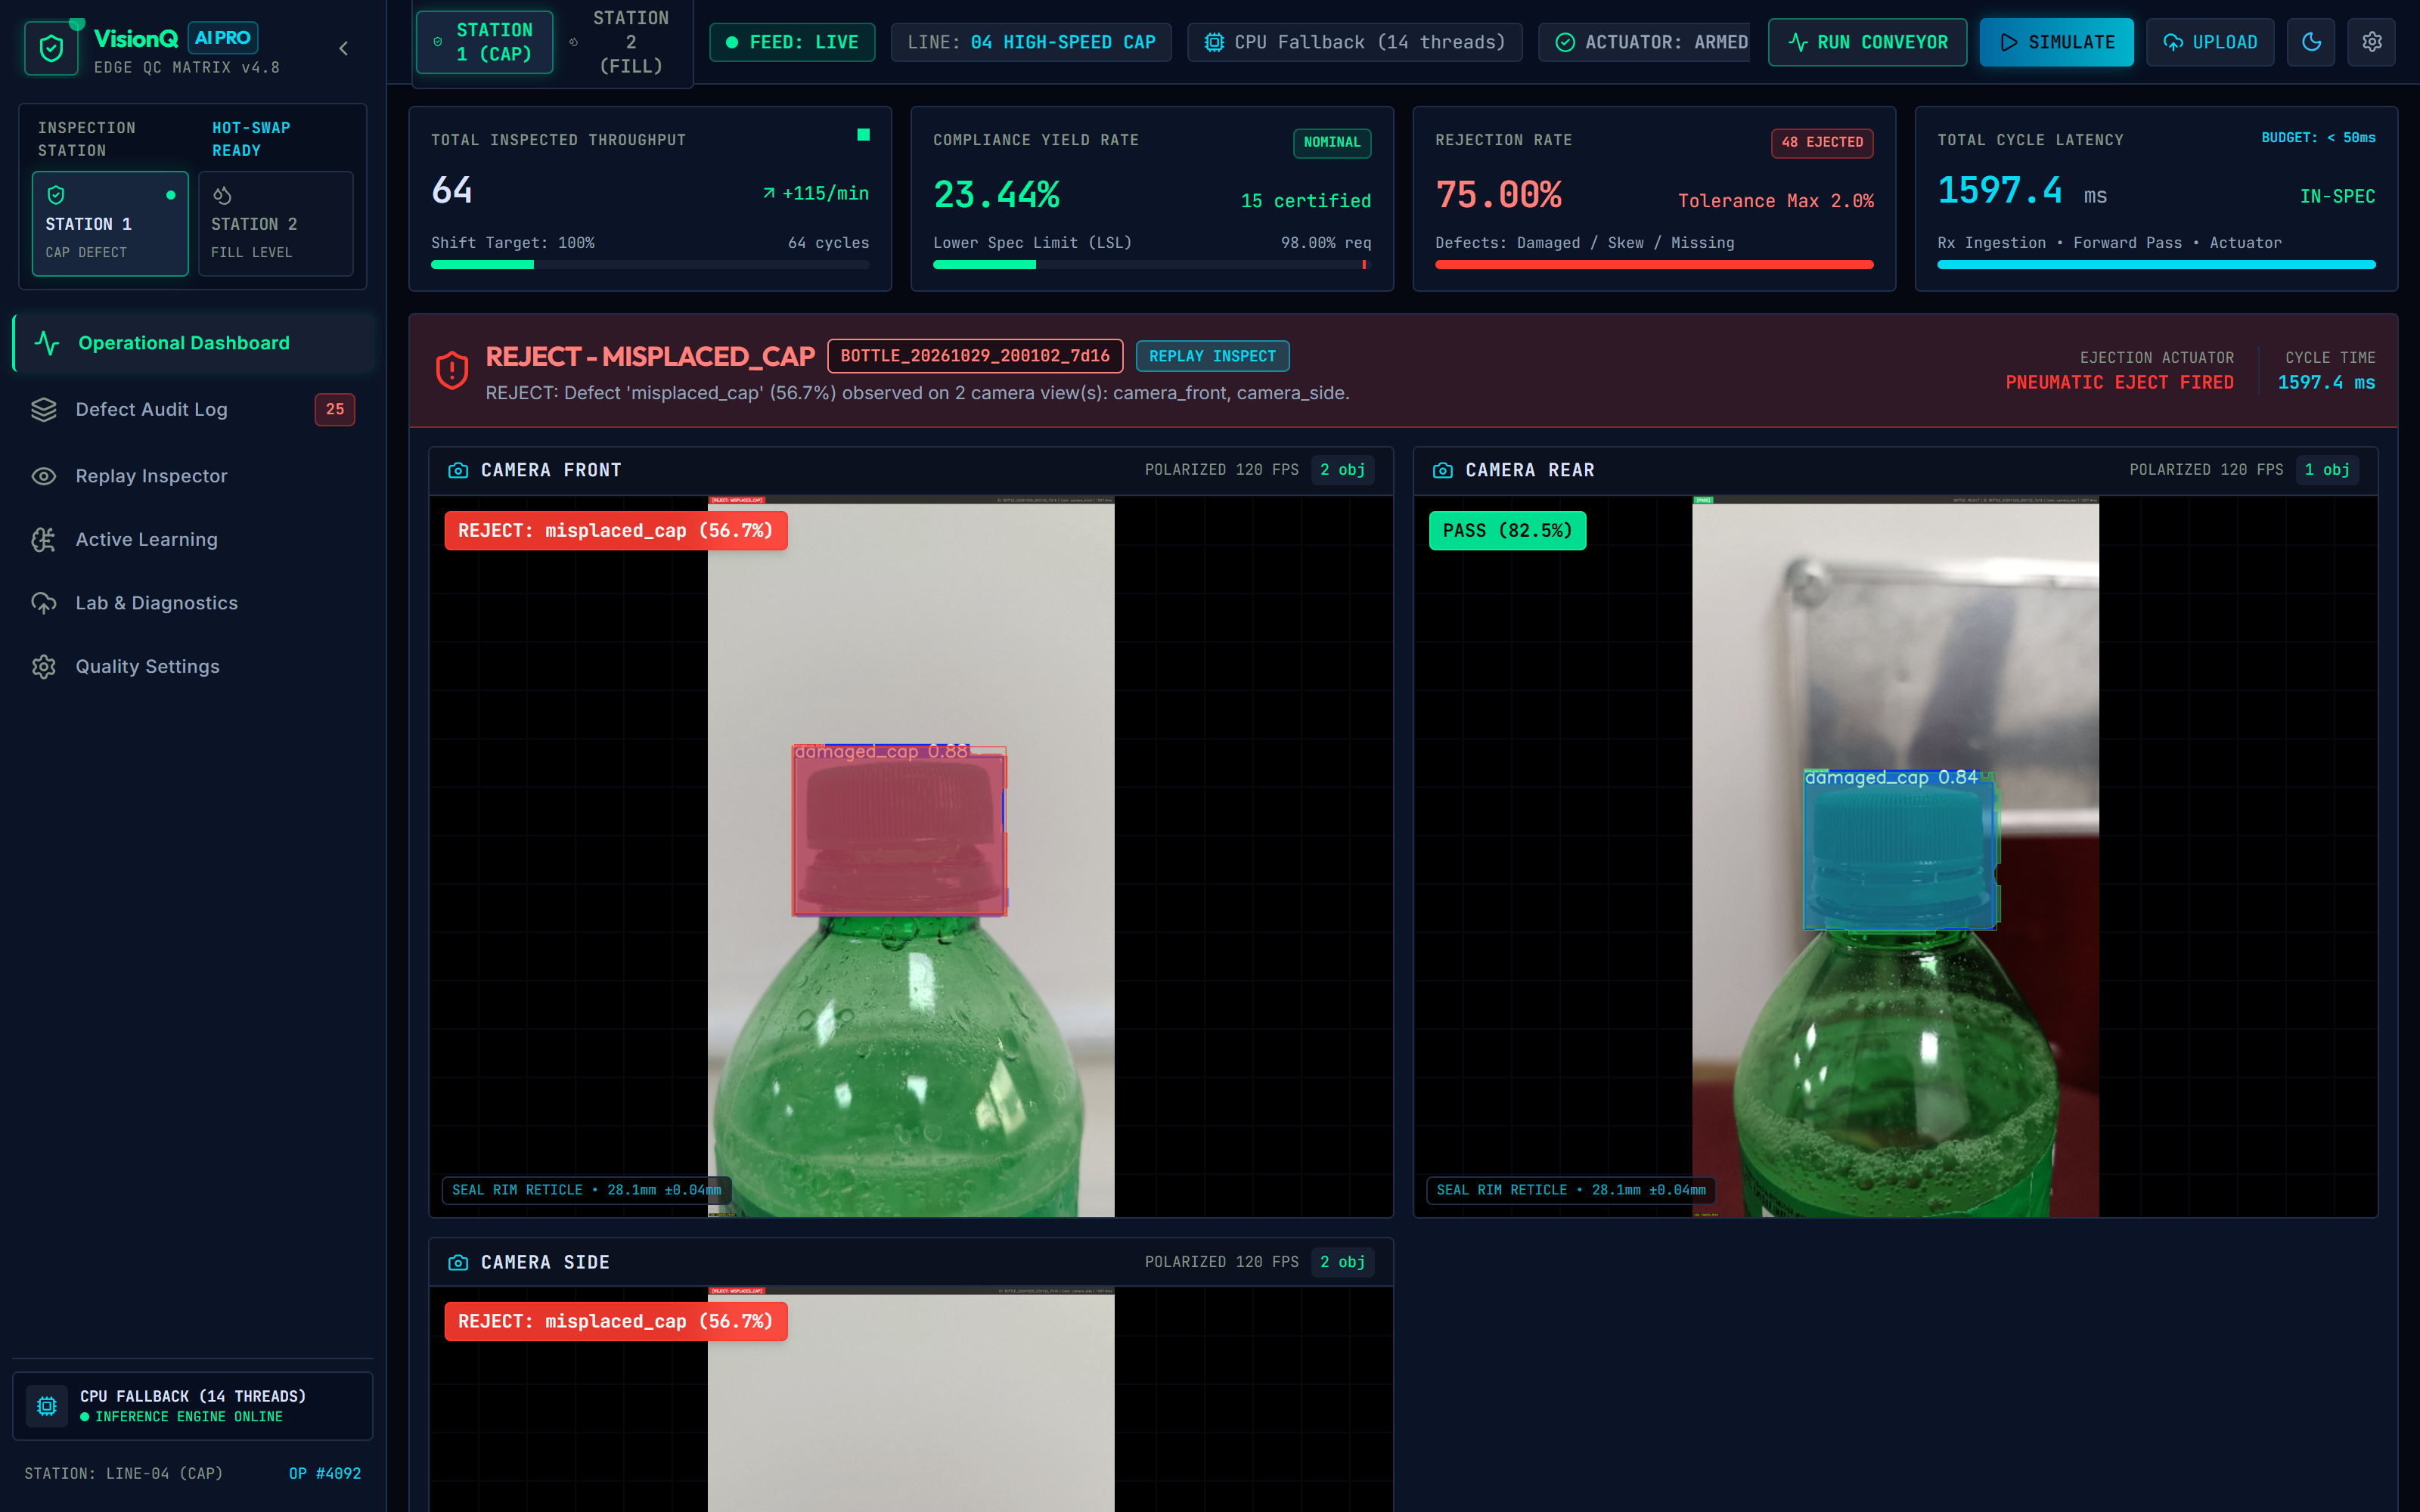
\includegraphics[width=\textwidth]{figures/dashboard_cap.png}
\caption[Station 1 (cap) dashboard after one simulated inspection]{Station 1 (cap) dashboard after one simulated inspection. The banner gives the bottle verdict (\texttt{REJECT}, misplaced cap on two of three views) and fires the reject actuator; each camera panel shows its own per-view verdict, mask overlay, and detection count.}
\label{fig:dash-cap}
\end{figure}

\begin{figure}[htbp]
\centering
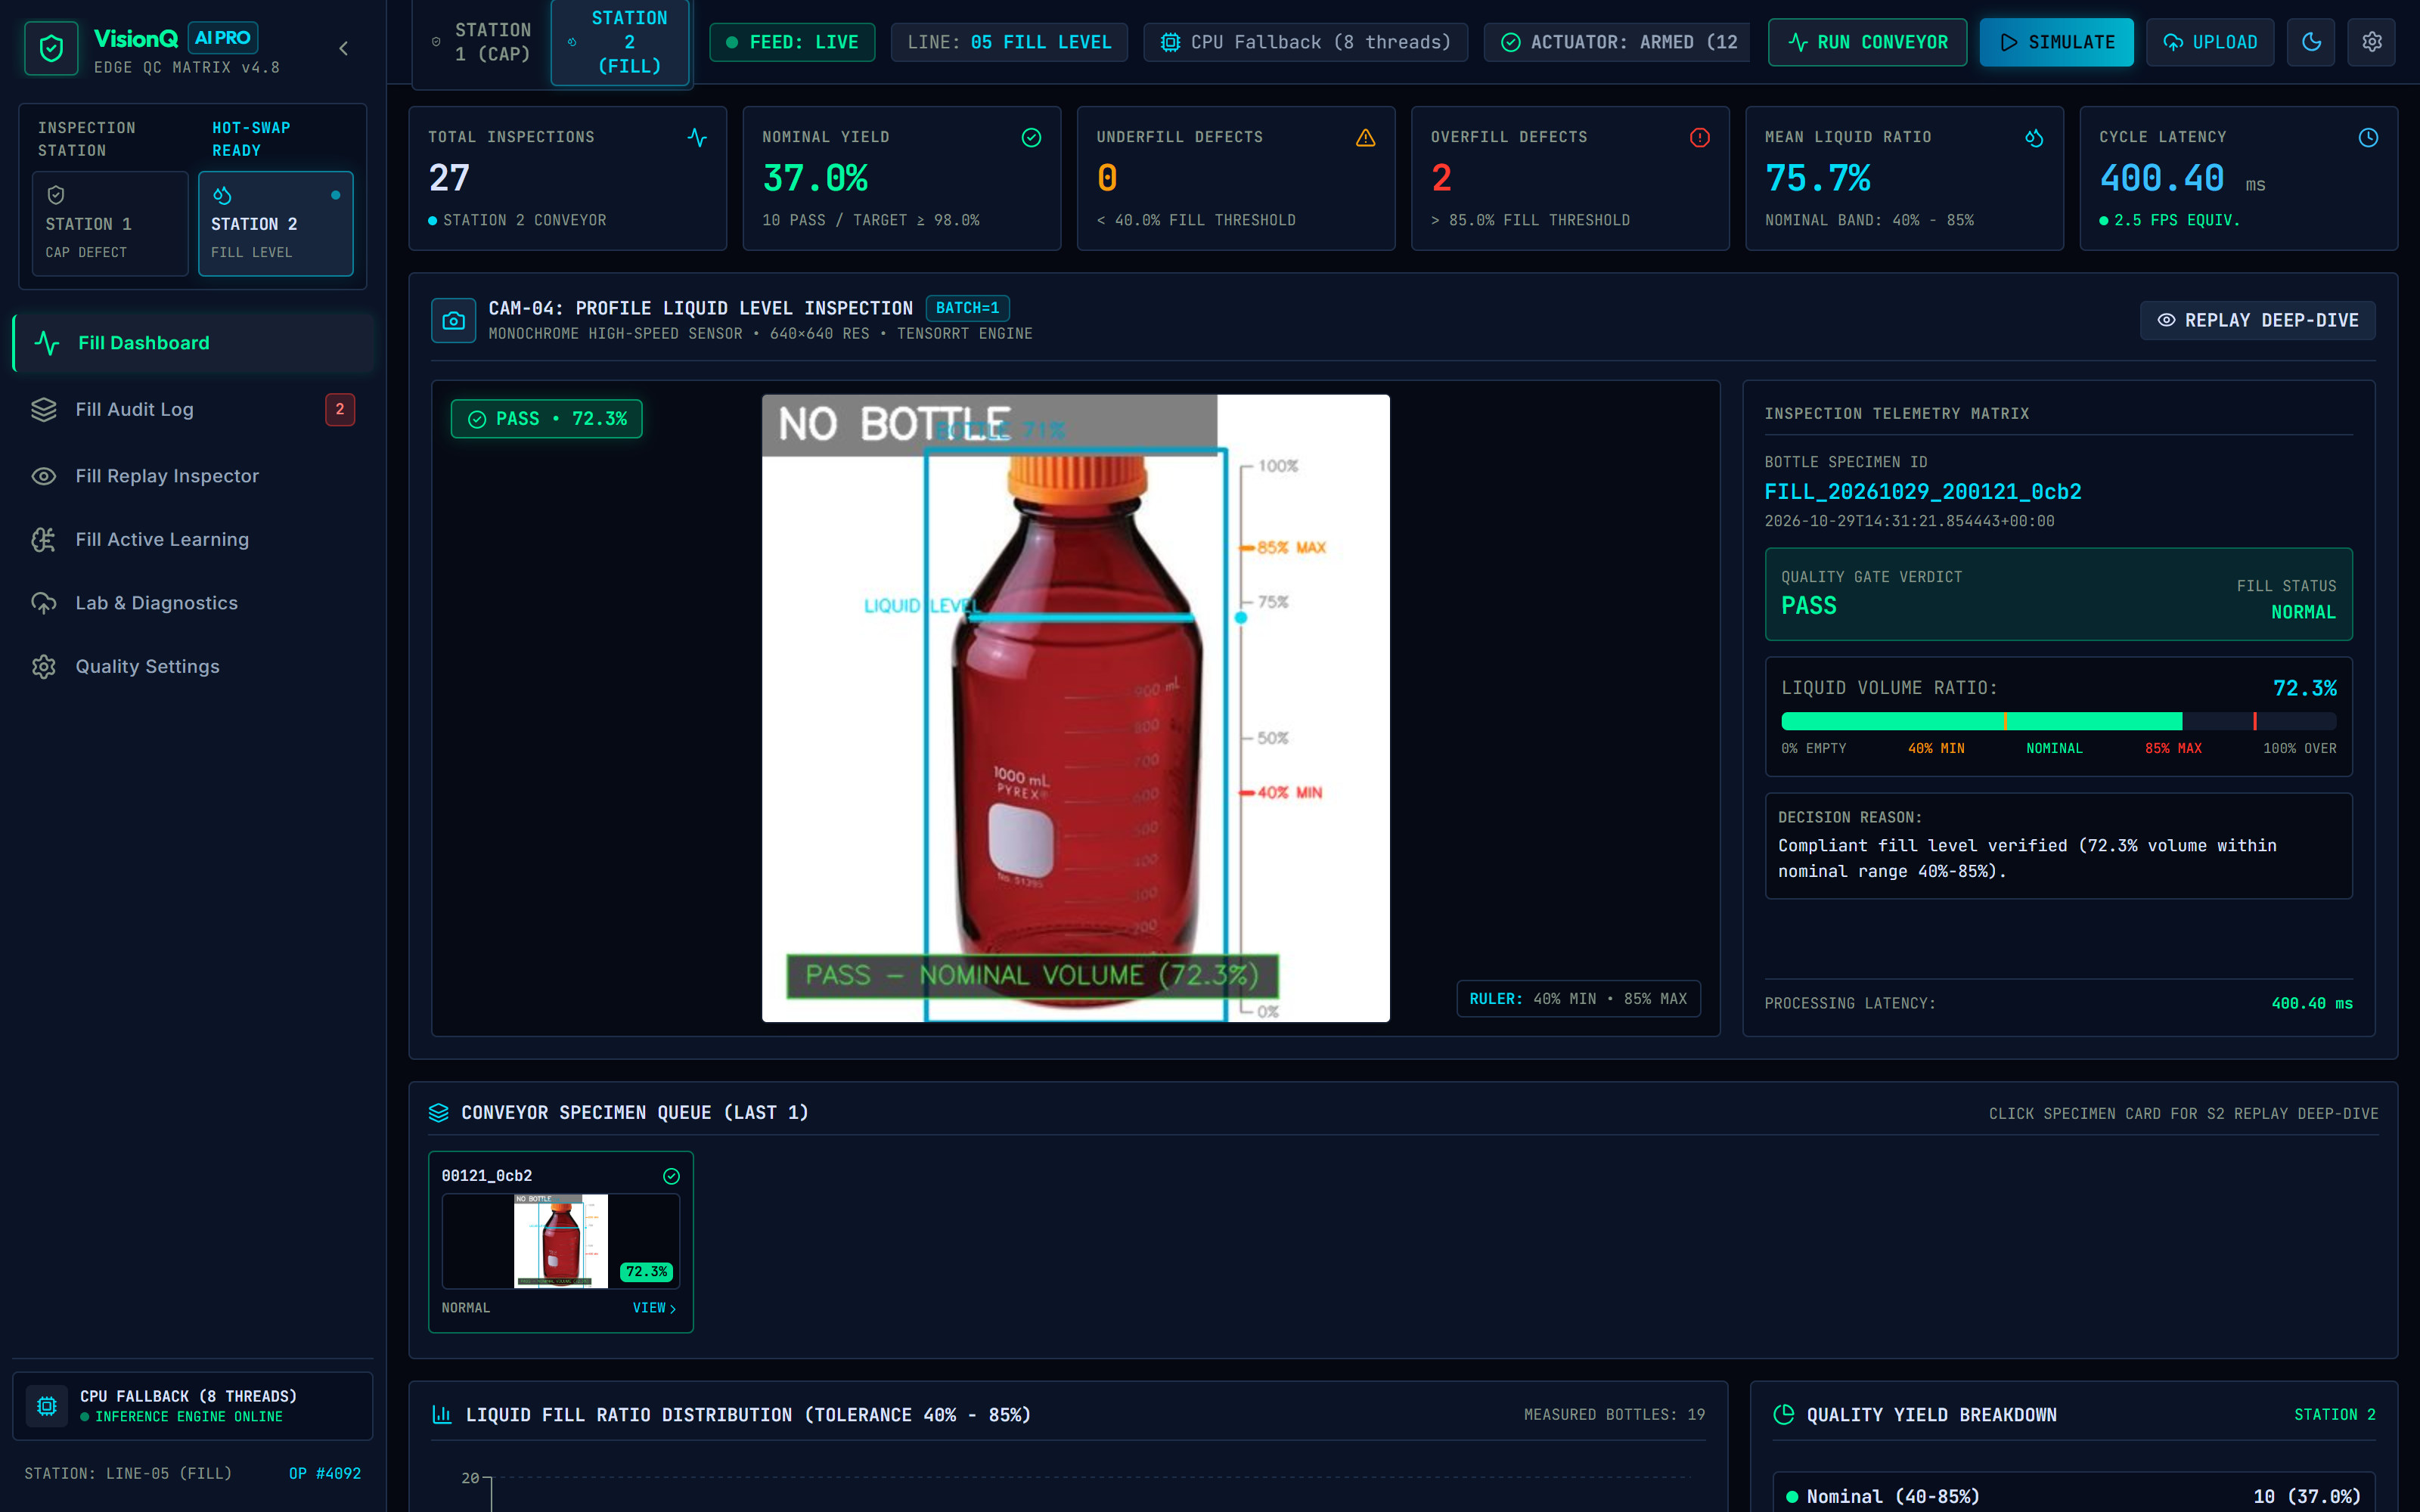
\includegraphics[width=\textwidth]{figures/dashboard_fill.png}
\caption[Station 2 (fill level) dashboard after one simulated inspection]{Station 2 (fill-level) dashboard after one simulated inspection. The frame shows the bottle box, the meniscus line, and the ruler with the 40\% and 85\% limits; the telemetry panel gives the fill ratio (72.3\%), the gate verdict (\texttt{PASS}), and the decision reason. The text banner at the top of the frame is part of the stored sample image.}
\label{fig:dash-fill}
\end{figure}

\begin{figure}[htbp]
\centering
\IfFileExists{figures/dashboard_label.png}{%
  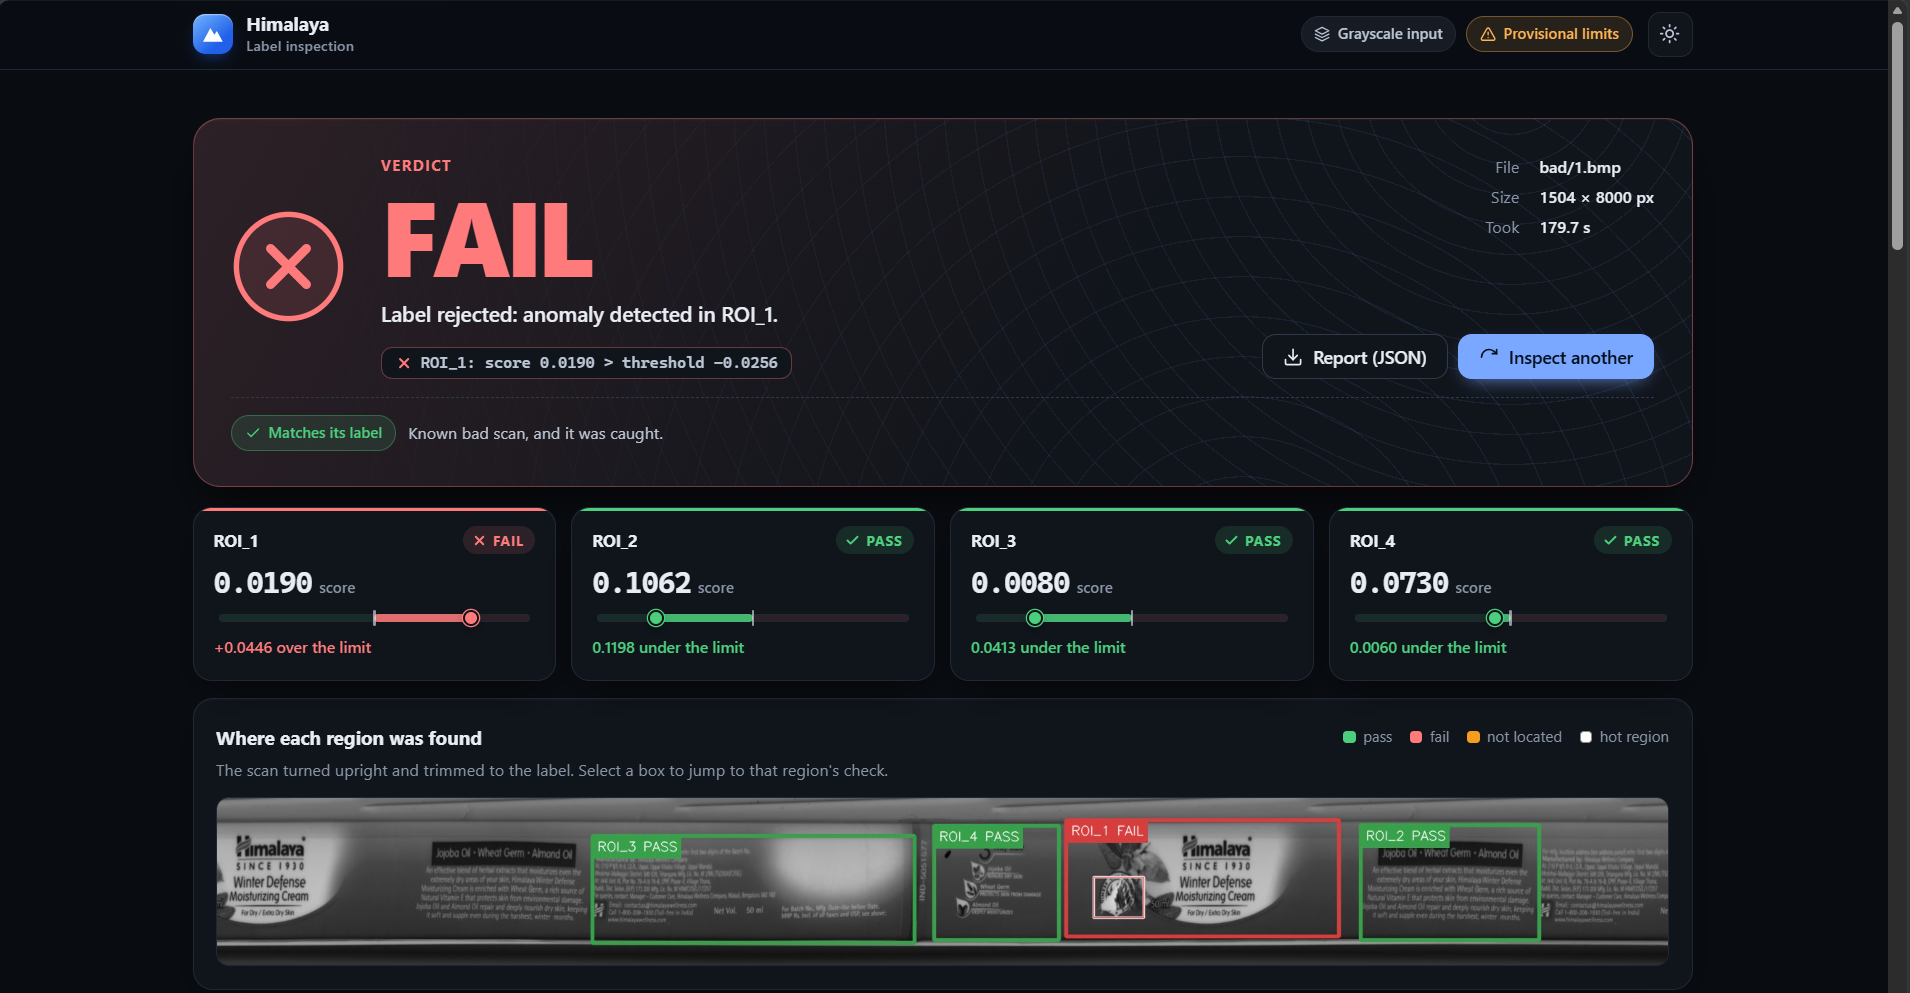
\includegraphics[width=\textwidth]{figures/dashboard_label.png}%
}{%
  \fbox{\parbox[c][6cm][c]{0.9\textwidth}{\centering Placeholder: add \texttt{figures/dashboard\_label.png}\\(label-inspection web application screenshot)}}%
}
\caption[Station 3 (label) inspection application]{Station 3 (label prototype) upload-and-inspect application: label verdict, per-region scores, and anomaly heatmaps for one NSC scan.}
\label{fig:dash-label}
\end{figure}

\subsection{Engine export and deployment}
\label{sec:deploy-impl}
Each PyTorch checkpoint is exported to ONNX and compiled to a TensorRT FP16 engine on the target GPU the first time the station loads. Algorithm~\ref{alg:engine} gives the procedure. The cap engine has a dynamic batch profile (optimum 3, maximum 4), so the three views of a bottle share one execution followed by NMS per view; the two fill engines have a static batch of 1 at 640\,px. Engines are cached under a version tag; changing the tag or setting a force-recompile flag rebuilds them. If no compatible GPU is present, the service falls back to ONNX Runtime and then to PyTorch. All paths come from environment variables resolved against the repository root, so the same code runs natively and in Docker, where the variables point at bind-mounted host folders.

\begin{algorithm}[htbp]
\caption{Engine load with versioned cache and fallback}
\label{alg:engine}
\begin{algorithmic}[1]
\Require Checkpoint path $p$, version tag $v$, batch profile $B$
\Ensure Loaded predictor
\If{CUDA available}
    \State $e \gets$ \texttt{<stem>\_<v>.engine} next to $p$
    \If{$e$ missing \textbf{or} force-recompile set}
        \State export $p \rightarrow$ ONNX $\rightarrow$ TensorRT FP16 with profile $B$ \Comment{minutes on first run}
    \EndIf
    \State load $e$; warm up (two single-image passes, plus a 3-view pass for the cap engine)
    \If{warm-up output shape $\neq$ expected batch} \State rebuild $e$ once \EndIf
\ElsIf{ONNX Runtime installed} \State load \texttt{.onnx}
\Else \State load \texttt{.pt} with PyTorch
\EndIf
\end{algorithmic}
\end{algorithm}

\subsection{Integration challenges}
Table~\ref{tab:challenges} records the main problems met during integration and how they were solved.

\begin{table}[htbp]
\centering
\caption{Integration challenges and solutions}
\label{tab:challenges}
\begin{tabularx}{\textwidth}{|L{4.6cm}|X|}
\hline
\textbf{Challenge} & \textbf{Solution} \\ \hline
TensorRT engine built with static batch 1 silently ran the three views one by one & Dynamic batch profile at export, batched warm-up check, automatic rebuild on shape mismatch. \\ \hline
Engines from one machine fail on another GPU & Compile on the target at first start; cache with version tag. \\ \hline
Two stations' engines in one 24\,GB GPU & Lazy load of Station 2, explicit unload/load on switch, inference and engine locks. \\ \hline
Inference blocking the web server & Thread-pool execution of all inference calls. \\ \hline
Host paths differ between machines and Docker & Environment-driven paths resolved against the repository root; Compose maps host folders to fixed container paths. \\ \hline
Label models fed the wrong colour mode & Threshold files record the input mode and score statistic; the CLI and web app refuse mismatched settings. \\ \hline
\end{tabularx}
\end{table}

\section{Software Testing}
\label{sec:testing-validation}

Testing followed the layer structure. Each station has one test script per layer (ingestion, inference, gate, audit, visualiser, API), an in-process end-to-end test runs both stations and the station swap, a stress test drives the full Station 1 loop inside the container, and the label prototype has 30 model-free unit tests for localisation, explainability, and the web app. Model accuracy was validated on held-out test splits that were not used for training or model selection (Chapter~\ref{ch:results}). Table~\ref{tab:test-results} lists representative test cases, including the failures.

\begin{table}[htbp]
\centering
\caption{Representative test cases}
\label{tab:test-results}
\begin{tabularx}{\textwidth}{|L{3.4cm}|L{3.2cm}|L{2.8cm}|X|}
\hline
\textbf{Test case} & \textbf{Input} & \textbf{Expected} & \textbf{Actual} \\ \hline
Cap gate, held-out test & 354 test images, FP16 engine & FAR $\leq3\%$, FRR $\leq7\%$ & 0/153 and 0/201 (Passed) \\ \hline
FP16 vs FP32 accuracy & Test split & $|\Delta\mAP|<0.01$ & $\leq0.0013$ overall (Passed) \\ \hline
Station swap & Cap$\rightarrow$fill$\rightarrow$cap in one process & Engines released and reloaded & Passed (in-process, CPU/ONNX) \\ \hline
Fill verdict agreement & 41 meniscus test images & $\geq0.93$ & 34/35 = 0.971 (Passed) \\ \hline
Fill, multi-bottle rack frames & 4 rack frames & Graceful handling & No bottle found $\Rightarrow$ \texttt{INSPECTION\_FAILED} (by design) \\ \hline
Closed loop at 300 bottles/min & 500 unpaced cycles & p50 $\leq200$\,ms & 299\,ms (Failed: storage-bound) \\ \hline
Paced run, 150 bottles/min & 300 cycles & 150 bottles/min & 126.7 bottles/min (Failed) \\ \hline
Database integrity under load & 800 cycles in total & No failed writes & 0 failures (Passed) \\ \hline
Label localisation & 120 NSC scans & All 4 ROIs found & 480/480 (Passed) \\ \hline
Label overlap rule & 120 NSC scans & No false re-assignment & Rule never fired (Passed) \\ \hline
Label ROI\_4 precision & 35 held-out crops & High precision & 57.9\% (Open issue) \\ \hline
\end{tabularx}
\end{table}
